\lstset{
	language = Matlab,
	frame = single,
	showstringspaces=false,
	%basicstyle=\ttfamily,
	basewidth={0.55em,0.55em},
	literate={а}{{\selectfont\char224}}1
	{б}{{\selectfont\char225}}1
	{в}{{\selectfont\char226}}1
	{г}{{\selectfont\char227}}1
	{д}{{\selectfont\char228}}1
	{е}{{\selectfont\char229}}1
	{ё}{{\"e}}1
	{ж}{{\selectfont\char230}}1
	{з}{{\selectfont\char231}}1
	{и}{{\selectfont\char232}}1
	{й}{{\selectfont\char233}}1
	{к}{{\selectfont\char234}}1
	{л}{{\selectfont\char235}}1
	{м}{{\selectfont\char236}}1
	{н}{{\selectfont\char237}}1
	{о}{{\selectfont\char238}}1
	{п}{{\selectfont\char239}}1
	{р}{{\selectfont\char240}}1
	{с}{{\selectfont\char241}}1
	{т}{{\selectfont\char242}}1
	{у}{{\selectfont\char243}}1
	{ф}{{\selectfont\char244}}1
	{х}{{\selectfont\char245}}1
	{ц}{{\selectfont\char246}}1
	{ч}{{\selectfont\char247}}1
	{ш}{{\selectfont\char248}}1
	{щ}{{\selectfont\char249}}1
	{ъ}{{\selectfont\char250}}1
	{ы}{{\selectfont\char251}}1
	{ь}{{\selectfont\char252}}1
	{э}{{\selectfont\char253}}1
	{ю}{{\selectfont\char254}}1
	{я}{{\selectfont\char255}}1
	{А}{{\selectfont\char192}}1
	{Б}{{\selectfont\char193}}1
	{В}{{\selectfont\char194}}1
	{Г}{{\selectfont\char195}}1
	{Д}{{\selectfont\char196}}1
	{Е}{{\selectfont\char197}}1
	{Ё}{{\"E}}1
	{Ж}{{\selectfont\char198}}1
	{З}{{\selectfont\char199}}1
	{И}{{\selectfont\char200}}1
	{Й}{{\selectfont\char201}}1
	{К}{{\selectfont\char202}}1
	{Л}{{\selectfont\char203}}1
	{М}{{\selectfont\char204}}1
	{Н}{{\selectfont\char205}}1
	{О}{{\selectfont\char206}}1
	{П}{{\selectfont\char207}}1
	{Р}{{\selectfont\char208}}1
	{С}{{\selectfont\char209}}1
	{Т}{{\selectfont\char210}}1
	{У}{{\selectfont\char211}}1
	{Ф}{{\selectfont\char212}}1
	{Х}{{\selectfont\char213}}1
	{Ц}{{\selectfont\char214}}1
	{Ч}{{\selectfont\char215}}1
	{Ш}{{\selectfont\char216}}1
	{Щ}{{\selectfont\char217}}1
	{Ъ}{{\selectfont\char218}}1
	{Ы}{{\selectfont\char219}}1
	{Ь}{{\selectfont\char220}}1
	{Э}{{\selectfont\char221}}1
	{Ю}{{\selectfont\char222}}1
	{Я}{{\selectfont\char223}}1
}

\newpage
\section*{Постановка задания}
\addcontentsline{toc}{section}{\tocsecindent{Постановка задания}}
\large
\textbf{Цель работы:} построение гистограммы и эмпирической функции распределения.\\
\textbf{Содержание работы:}
\\
1. Для выборки объема $n$ из генеральной совокупности $X$ реализовать в виде программы на ЭВМ:

 а) вычисление максимального значения $M_{max}$ и минимального значения $M_{min}$;

	б) размаха $R$ выборки;

	в) вычисление оценок $\hat\mu$ и $S^2$ математического ожидания $MX$ и дисперсии $DX$;
	
	г) группировку значений выборки в $m = [log_2 n] + 2$ интервала;
	
	д) построение на одной координатной плоскости гистограммы и графика функции плотности распределения вероятностей нормальной случайной величины с математическим
	ожиданием $\hat\mu$ и дисперсией $S^2$;
	
е) построение на другой координатной плоскости графика эмпирической функции распределения и функции распределения нормальной случайной величины с математическим
ожиданием $\hat\mu$ и дисперсией $S^2$.
\\
2. Провести вычисления и построить графики для выборки из индивидуального варианта.
\textbf{Содержание отчета}

1. формулы для вычисления величин $M_{max}$, $M_{min}$, $R$, $\hat\mu$, $S^2$;

2. определение эмпирической плотности и гистограммы;

3. определение эмпирической функции распределения;

4. текст программы;

5. результаты расчетов для выборки 1 из индивидуального варианта.

\section*{Теоретическая часть}
\addcontentsline{toc}{section}{\tocsecindent{Теоретическая часть}}

\section*{Формулы для вычисления величин}
Ниже представлены формулы для вычисления величин.
\\
\textbf{Минимальное значение выборки}

\begin{equation}
M_{\min} = \min \{ x_1, \dots, x_n\}, \quad \text{где} (x_1, \dots, x_n) - \text{реализация случайной выборки.}
\end{equation}
\\ \textbf{Максимальное значение выборки}

\begin{equation}
M_{\max} = \max \{ x_1, \dots, x_n\}, \quad \text{где} (x_1, \dots, x_n) - \text{реализация случайной выборки.}
\end{equation}
\\ \textbf{Размах выборки}

\begin{eqnarray}
R = M_{\max} - M_{\min}, \quad \text{где } M_{\max} - \text{максимальное значение выборки}, \\ M_{\min} - \text{минимальное значение выборки}.
\end{eqnarray}
\\ \textbf{Оценка математического ожидания}

\begin{equation}
\hat{\mu}(\vec{X}_n) = \overline{X}_n = \frac{1}{n} \sum_{i = 1}^{n} X_i\,.
\end{equation}
\\
\textbf{Несмещённая оценка дисперсии}
\begin{equation}
S^2(\vec{X}_n) = \frac{n}{n - 1}\hat{\sigma}^2 = \frac{1}{n - 1}\sum_{i = 1}^{n} (X_i - \overline{X}_n)^2\,.
\end{equation}

\section*{Определения величин}

\textbf{Эмпирическая плотность и гистограмма}

\begin{defn}
	\emph{Эмпирической плотностью распределения случайной выборки $\vec{X}_n$} называют функцию
	\begin{equation}
	f_n(x) =
	\begin{cases}
	\frac{n_i}{n \, \Delta}, &x \in J_i,\; i = \overline{1, m};\\
	0, &\text{иначе}.
	\end{cases}, \quad \text{где}
	\end{equation}
	\begin{enumerate}
		\item $J_i,\, i = \overline{1; m}$, --- полуинтервал из $J = [x_{(1)}, x_{(n)}]$, где 
		\begin{align}
		&x_{(1)} = \min\{ x_1, \dots, x_n \}, &x_{(n)} = \max\{ x_1, \dots, x_n \};
		\end{align}
		при этом все полуинтервалы, кроме последнего, не содержат правую границу т.\,е.
		\begin{align}
		&J_i = [a_i, a_{i+1}), i = \overline{1; m - 1};
		\\
		&J_{m} = [a_{m}, a_{m+1}];
		\end{align}
		где \begin{align}a_i = x_{(1)} + (i-1)\cdot\Delta, i = \overline{1;m+1};\end{align}
		\item $m$ --- количество полуинтервалов интервала $J = [x_{(1)}, x_{(n)}]$;
		\item $\Delta$ --- длина полуинтервала $J_i$, $i = \overline{1, m}$ равная
		\begin{equation}
		\Delta = \frac{x_{(n)} - x_{(1)}}{m} = \frac{|J|}{m};
		\end{equation}
		\item $n_i$ --- количество элементов выборки в полуинтервале $J_i$, $i = \overline{1, m}$;
		\item $n$ --- количество элементов в выборке.
		
	\end{enumerate}
\end{defn}

\begin{defn}
	График функции $f_n(x)$ называют гистограммой. \\
	\\ \textbf{Эмпирическая функция распределения}
\end{defn}


\begin{enumerate}
	\item $\vec{X}_n = (X_1, \ldots, X_n)$ --- случайная выборка;
	\item $\vec{x}_n = (x_1, \dots, x_n)$ --- реализация случайной выборки $\vec{X}_n$;
	\item $n(x, \vec{x}_n)$ --- количество элементов выборки $\vec{x}_n$, которые меньше $x$.
\end{enumerate}

\begin{defn}
	\emph{Эмпирической функцией распределения} называют функцию
	\begin{equation}
	F_n\colon \mathbb{R} \to \mathbb{R}, \quad F_n(x) = \frac{n(x, \vec{x}_n)}{n}
	\end{equation}
\end{defn}
\begin{rem}
	$F_n(x)$ обладает всеми свойствами функции распределения. При этом она кусочно-постоянна и принимает значения 
	\[
	0, \frac{1}{n}, \frac{2}{n}, \ldots, \frac{(n-1)}{n}, 1
	\]
\end{rem}
\begin{rem}
	Если все элементы вектора $\vec{x}_n$ различны, то
	\begin{equation}
	F_n(x) = 
	\begin{cases}
	0, & x \leq x_{(1)}; \\
	\frac{i}{n}, & x_{(i)} < x \leq x_{(i+1)},\; i = \overline{1, n-1}; \\
	1, & x > x_{(n)}.
	\end{cases}
	\end{equation}
\end{rem}

\section*{Листинг программы}
\addcontentsline{toc}{section}{\tocsecindent{Листинг программы}}

\begin{lstlisting}[language=Matlab, caption=Текст программы]
function lab1
clear all;

% считываем из файла
X = csvread('data.txt')

% получаем вариационный ряд и его длину
X = sort(X)
n = size(X, 2)

% максимальный и минимальный элементы, размах
X_min = X(1)
X_max = X(end)
R = X_max - X_min

% вычисление оценок mu и S2 математического ожидания MX и дисперсии DX
mu = mean(X)
S2 = var(X)

% группировкa значений выборки в m = [log2 n] + 2 интервала
m = floor(log2(n) + 2)
h = R / m
intervals = zeros(m, 2)

% получаем границы интервалов
for i = 1:m
intervals(i,1) = X(1) + h * i;
end 

% заполняем интервалыы
i = 1, j = 1
border = X(1) + h

while i < n
if X(i) >= border && border < X(n) && j < m
border = border + h
j = j + 1
continue % на случай, если в интервале нет чисел
end

intervals(j, 2) = intervals(j, 2) + 1
i = i + 1
end

intervals(m, 2) = intervals(m, 2) + 1; % последний элемент

% гистограмма и ф-я плотности
gist = zeros(m, 2)
gist(1, 1) = (X(1) + intervals(1, 1))./2

% интервалы для гистограммы (значения по x)
for i = 2:m
gist(i, 1) = (intervals(i - 1, 1) + intervals(i, 1))./2
end

% значения по y для гистограммы 
for i = 1:m
y = intervals(i, 2)
y = y / (n * h)
gist(i,2) = y
end

% функция плотности нормальной случайной величины
f = 1 / sqrt(2 * pi * S2) * exp(-power((X - mu), 2) / (2 * S2))

% график гистограммы и функции плотности
bar(gist(:,1), gist(:,2), 1)
hold on
plot (X, f, 'r'), grid
figure()

% эмпирическая ф-я плотности и ф-я распределения
empir = zeros(1, n+2)
empir(1) = X(1) - 1

for i = 1:n
empir(i + 1) = X(i)
end

empir(n + 2) = X(n) + 1

% вычисление интервалов для функций
n_emp = length(empir)
Mmin = min(empir)
Mmax = max(empir)
step = (Mmax - Mmin) / n_emp
Xn = Mmin : step : Mmax

% вычисление значений для эмпирической функции
E = zeros(n_emp, 1)

for i = 1:n_emp
count = 0

for j = 1:n
if X(j) <= empir(i)
count = count + 1
end
end

E(i) = count / n
end

% функция распределения нормальной случайной величины
F = 1/2 * (1 + erf((Xn - mu) / sqrt(2 * S2)))

% графики
plot(Xn, F, "--"), grid
hold on
stairs(empir, E), grid
end
\end{lstlisting}

\section*{Результаты работы и графики}
\addcontentsline{toc}{section}{\tocsecindent{Результаты работы и графики}}

\begin{align}
M_{max} = -15.270\\
M_{min} = -19.470\\
R = 4.2\\
\hat\mu = -17.589\\
S^2 = 0.7286
\end{align}

\begin{align}
\text{Интервалы: } [-19.470, -18.945) [-18.945, -18.420) [-18.420, -17.895) [-17.895, -17.370)\\ \nonumber
[-17.370, -16.845) [-16.845, -16.320) [-16.320, -15.795) [-15.795, -15.270].
\end{align}

\begin{figure}[h]
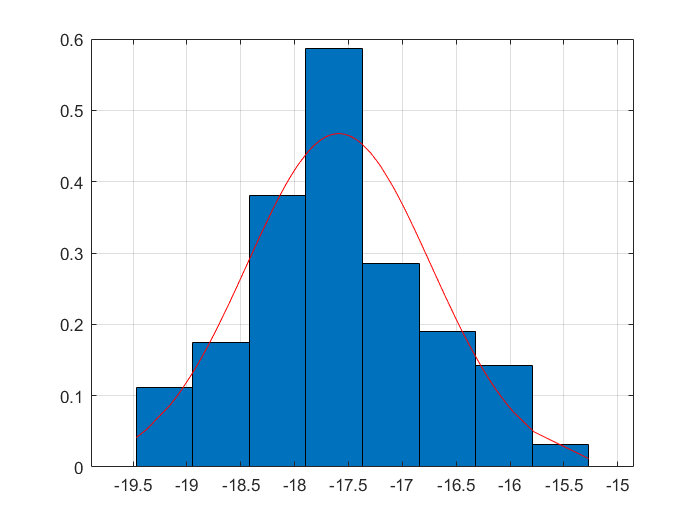
\includegraphics{untitled}
\caption{Гистограмма и график функции плотности распределения вероятностей}
\label{fig:image}
\end{figure}

\begin{figure}[h]
	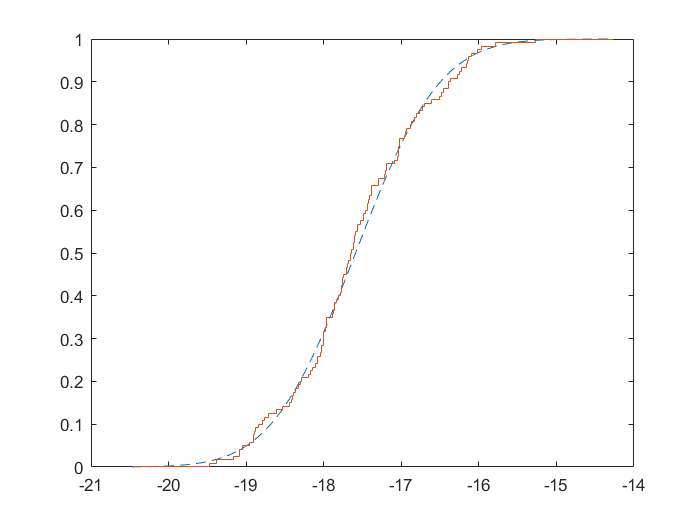
\includegraphics{untitled2}
	\caption{График эмпирической функции распределения и функции распределения}
	\label{fig:image1}
\end{figure}